\documentclass[9pt]{beamer}

% beamerthemeFeng.sty
% style file for beamer presentation

% tikz is used to ``draw'' title page and other templates in beamer
\usepackage{tikz,etoolbox}
\usetikzlibrary{shapes,arrows}

\definecolor{UWBlack}{HTML}{000000}
\definecolor{UWWhite}{HTML}{FFFFFF}


\definecolor{UWMathPinkL1}{HTML}{FFBEEF}
\definecolor{UWMathPinkL2}{HTML}{FF63AA}
\definecolor{UWMathPinkL3}{HTML}{DF2498}
\definecolor{UWMathPinkL4}{HTML}{C60078}
\definecolor{UWGrayL1}{HTML}{DFDFDF}
\definecolor{UWGrayL2}{HTML}{A2A2A2}
\definecolor{UWGrayL3}{HTML}{787878}
\definecolor{UWGrayL4}{HTML}{000000}
\definecolor{UWGoldL1}{HTML}{FFFFAA}
\definecolor{UWGoldL2}{HTML}{FFEA3D}
\definecolor{UWGoldL3}{HTML}{FFD54F}
\definecolor{UWGoldL4}{HTML}{E4B429}

\definecolor{carrot}{HTML}{EE693F}
\definecolor{ivory}{HTML}{F1F3CE}
\definecolor{emerald}{HTML}{265C00}
\definecolor{turquise}{HTML}{5BC8AC}
\definecolor{peacockblue}{HTML}{1E656D}
\definecolor{spicy}{HTML}{B51D0A}
\definecolor{bluegreen}{HTML}{5F968E}
\definecolor{rust}{HTML}{9B4F0F}
\definecolor{burntorange}{HTML}{DE7A22}
\definecolor{sea}{HTML}{20948B}
\definecolor{lagoon}{HTML}{6AB187}


% Set colors for different components in a slide
\setbeamercolor{background canvas}{bg=UWWhite}
\setbeamercolor{author}{fg=UWGoldL3}
\setbeamercolor{institute}{fg=UWMathPinkL3}
\setbeamercolor{title}{fg=UWGrayL4}
\setbeamercolor{section in head/foot}{bg=UWBlack, fg=UWGoldL3}
\setbeamercolor{author in head/foot}{fg=UWGoldL3, bg=UWBlack}
\setbeamercolor{title in head/foot}{fg=UWBlack,bg=UWGoldL3}
\setbeamercolor{institute in head/foot}{fg=UWGoldL3, bg=UWBlack}
\setbeamercolor{navigation symbols}{fg=UWBlack}
\setbeamercolor{normal text}{fg=UWGrayL3}
\setbeamercolor{section in toc}{fg=emerald}
\setbeamercolor{subsection in toc}{fg=bluegreen}
\setbeamercolor{frametitle}{fg=UWMathPinkL2, bg=UWGrayL1}
\setbeamercolor{block title}{bg=emerald, fg=ivory}
\setbeamercolor{block body}{bg=peacockblue!20, fg=peacockblue}
\setbeamercolor{section number projected}{bg=turquise,fg=black}
\setbeamercolor{block title example}{fg=rust,
	bg= sea!40}
\setbeamercolor{block body example}{fg= burntorange,
	bg= lagoon!20}

\setbeamerfont{frametitle}{series=\bfseries} % bold frame title
\setbeamerfont{section number projected}{% bold TOC bullet
  family=\rmfamily,series=\bfseries,size=\normalsize}
  
% two common fields in conference presentations
\newcommand\jointwork[1]{\def\insertjointwork{#1}}
\newcommand\conference[1]{\def\insertconference{#1}}

% Title page style
\setbeamertemplate{title page}{
\begin{tikzpicture}[remember picture, overlay]
\fill[UWWhite]
  ([yshift=30pt]current page.west) rectangle (current page.south east);

\fill[UWBlack]
  ([yshift=30pt]current page.west) rectangle (current page.north east);

\node[anchor=east] at ([yshift=-50pt,xshift=-15pt]current page.north east)
  {
  
\includegraphics[width=0.3\linewidth]{./hselogo_fullsize_inverted.png}};

\node[anchor=north west] at ([yshift=-70pt,xshift=15pt]current page.north west) (institute)
	{
	\parbox[t]{.78\paperwidth}{
    \usebeamerfont{institute}\usebeamercolor[fg]{institute}\large\bfseries\insertinstitute}
    };
    
\node[anchor=west] at ([yshift=-45pt,xshift=15pt]current page.north west) (author)
	{
	\parbox[t]{.78\paperwidth}{
    \usebeamerfont{author}\usebeamercolor[fg]{author}\Large\bfseries \insertauthor}
    };


    
\node[anchor=north] at ([yshift=15pt]current page.center) (title)
	{
	\parbox[t]{\textwidth}{\huge\bfseries\centering
	\usebeamerfont{title}\usebeamercolor[fg]{title}\inserttitle}
	};
    
\node[anchor=north] at ([yshift=-40pt]current page.center) (jointwork)
	{
	\parbox[t]{\paperwidth}{\bfseries\centering\insertjointwork}
	};
	
\node[anchor=north] at ([yshift=40pt]current page.south) (jointwork)
	{
	\parbox[t]{\paperwidth}{\centering\insertconference}
	};
\end{tikzpicture}
}

\setbeamertemplate{headline} % add navigation to headline
{%
  \begin{beamercolorbox}{section in head/foot}
    \vskip5pt\bfseries
    \insertnavigation{\paperwidth}
    \vskip2pt
  \end{beamercolorbox}%
}


\renewcommand*{\slideentry}[6]{} % no solid circle in headline

% three-parts footline, color determined in beamer template
\setbeamertemplate{footline}
{
	\leavevmode % vertical mode is ended and horizontal mode is entered. In vertical mode, TeX stacks horizontal boxes vertically, whereas in horizontal mode, they are taken as part of the text line. 
	\begin{beamercolorbox}[wd=.333333\paperwidth,ht=2.5ex,dp=1.125ex,
      leftskip=.3cm,rightskip=.3cm plus1fil]{author in head/foot}
		\usebeamerfont{author in head/foot}\insertshortauthor
    \end{beamercolorbox}%
    \begin{beamercolorbox}[wd=.333333\paperwidth,ht=2.5ex,dp=1.125ex,
      leftskip=.3cm,rightskip=.3cm plus1fil,center]{title in head/foot}
      {\usebeamerfont{title in head/foot}\insertshorttitle}
    \end{beamercolorbox}%
    \begin{beamercolorbox}[wd=.333333\paperwidth,ht=2.5ex,dp=1.125ex,
      leftskip=.3cm,rightskip=.3cm plus1fil]{institute in head/foot}
      \hfill    {\usebeamercolor[fg]{institute in head/foot}\insertshortinstitute}    
	\end{beamercolorbox}%
}

\setbeamertemplate{navigation symbols}{\bfseries\insertframenumber/\inserttotalframenumber}

\setbeamertemplate{sections/subsections in toc}[ball]

% make the itemize bullets pixelated >
\setbeamertemplate{itemize item}{
	\tikz{
		\draw[fill=spicy,draw=none] (0, 0) rectangle(0.075, 0.075);
		\draw[fill=spicy,draw=none] (0.075, 0.075) rectangle(0.15, 0.15);
		\draw[fill=spicy,draw=none] (0, 0.15) rectangle(0.075, 0.225);
	}
}

% make the subitems also pixelated >, but a little smaller and red
\setbeamertemplate{itemize subitem}{
	\tikz{
		\draw[fill=carrot,draw=none] (0, 0) rectangle(0.05, 0.05);
		\draw[fill=carrot,draw=none] (0.05, 0.05) rectangle(0.1, 0.1);
		\draw[fill=carrot,draw=none] (0, 0.1) rectangle(0.05, 0.15);
	}
}

\AtBeginEnvironment{block}{
	\setbeamertemplate{itemize item}{
		\tikz{
			\draw[fill=spicy,draw=none] (0, 0) rectangle(0.075, 0.075);
			\draw[fill=spicy,draw=none] (0.075, 0.075) rectangle(0.15, 0.15);
			\draw[fill=spicy,draw=none] (0, 0.15) rectangle(0.075, 0.225);
		}
	}

	\setbeamertemplate{itemize subitem}{
		\tikz{
			\draw[fill=carrot,draw=none] (0, 0) rectangle(0.05, 0.05);
			\draw[fill=carrot,draw=none] (0.05, 0.05) rectangle(0.1, 0.1);
			\draw[fill=carrot,draw=none] (0, 0.1) rectangle(0.05, 0.15);
		}
	}
}

\setbeamertemplate{blocks}[rounded][shadow=false]

\setbeamercovered{invisible}

\usefonttheme[onlymath]{serif} % change the math font theme

\AtBeginEnvironment{theorem}{%
  \setbeamercolor{block title}{bg=peppercorn, fg=pearl}
  \setbeamercolor{block body}{bg=parsnip, fg=spicy}
}

\setbeamertemplate{caption}[numbered]

% set color scheme in different parts 
% please refer to beamer cheatsheet below for details
% http://www.cpt.univ-mrs.fr/~masson/latex/Beamer-appearance-cheat-sheet.pdf

\usepackage{wrapfig}

\usepackage{tikz}
\usepackage[main=russian,english]{babel}
\usepackage[utf8]{inputenc}
\usepackage[T1,T2A]{fontenc}

\usepackage{xcolor, color, soul}
\sethlcolor{red}

\usepackage{tabularx}
\usepackage{geometry}
\usepackage{wrapfig}

\usepackage{subfig}

\usepackage{movie15}

\usepackage{subfig}
\usepackage{tabularx}
\usepackage{booktabs}
\usepackage{pifont}

\newcommand{\cmark}{\ding{51}}
\newcommand{\xmark}{\ding{55}}
\usepackage{xcolor}

\usepackage[backend=biber,style=numeric,urldate=long,maxbibnames=99,sorting=none]{biblatex}
\addbibresource{refs.bib}

\title[\textbf{}]{Оптимизация размера сенсоров для физики элементарных частиц} % The short title appears at the bottom of every slide, the full title is only on the title page

\author[\textbf{Зиманов Алихан}]
{Зиманов Алихан} % Your name

\institute[\textbf{ВШЭ}] % Your institution as it will appear on the bottom of every slide, may be shorthand to save space
{Исследовательский проект\\
ВКР % Your institution for the title page
}

\jointwork{Научный руководитель Болдырев А.С.}
\conference{Москва, 2024}

%===== Uncomment the following if you wish to use references
%\usepackage[backend=bibtex,citestyle=authoryear-icomp,natbib,maxcitenames=1]{biblatex}
%\addbibresource{bibfile.bib}

% use this so appendices' page numbers do not count
\usepackage{appendixnumberbeamer}

\begin{document}

% Title page, navigation surpressed, no page number
{
\beamertemplatenavigationsymbolsempty
\begin{frame}[plain]
\titlepage
\end{frame}
}

% TOC, navigation surpressed, no page number
{
\beamertemplatenavigationsymbolsempty
\defbeamertemplate*{headline}{miniframes theme no subsection no content}
{ \begin{beamercolorbox}{section in head/foot}
    \vskip\headheight
  \end{beamercolorbox}}
\begin{frame}{Содержание} 
\tableofcontents 
\end{frame} 
}

\addtocounter{framenumber}{-2}

\section{Введение}

\begin{frame}{Постановка задачи}
    \begin{figure}
        \centering
        \subfloat{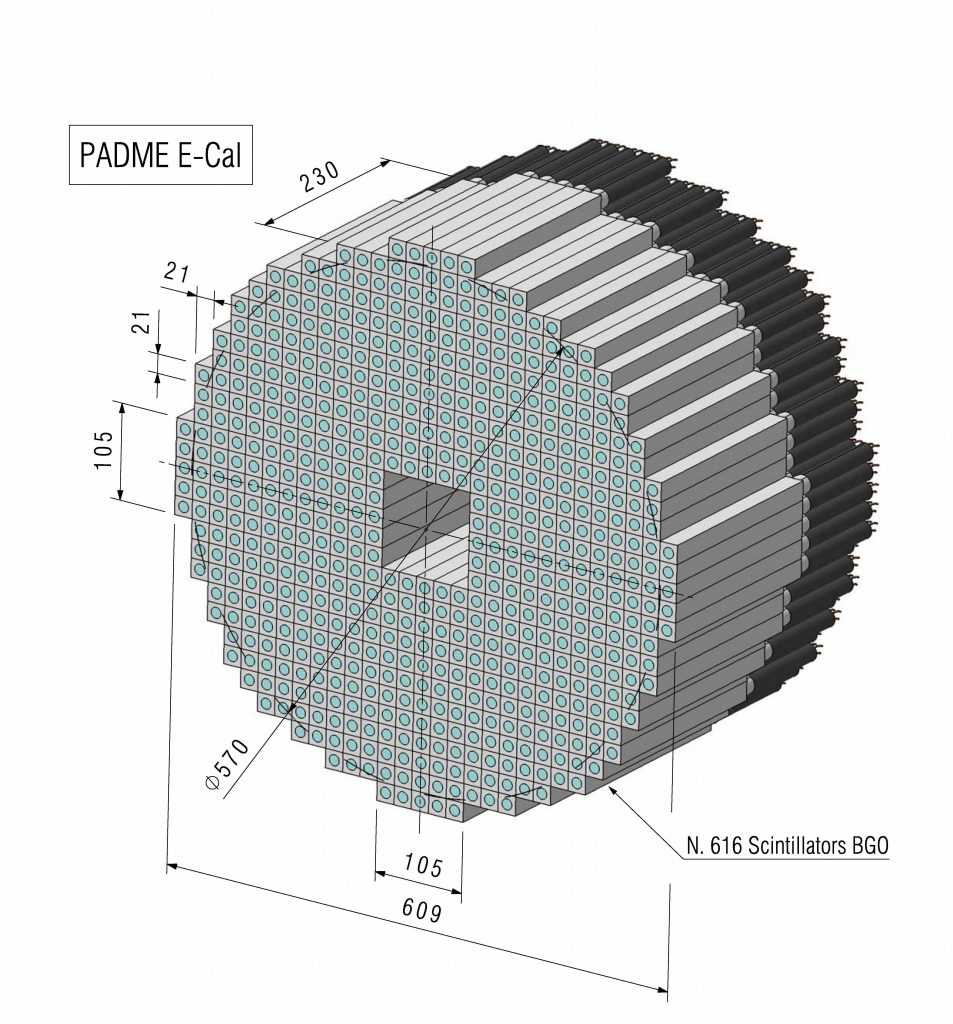
\includegraphics[width=0.45\textwidth]{../report/graphics/ecal_big.jpg}}\qquad
        \subfloat{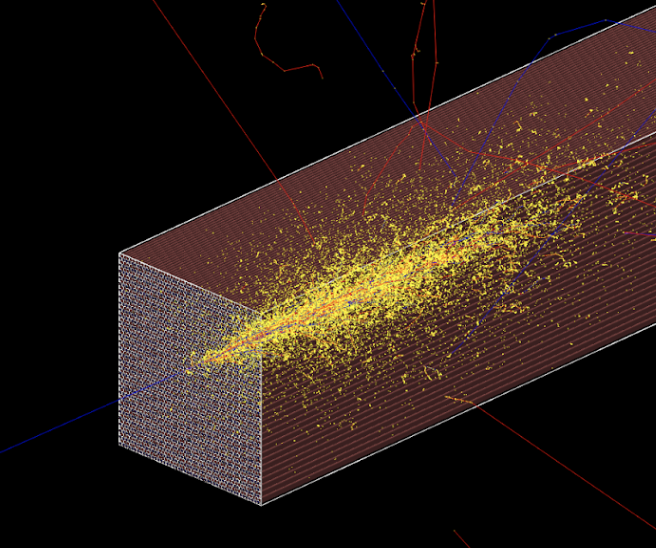
\includegraphics[width=0.45\textwidth]{../report/graphics/shower.png}}
        \caption{Электромагнитный калориметр PADME и симуляция электромагнитного ливня с помощью GEANT4.}
    \end{figure}
\end{frame}

\begin{frame}{Актуальность работы}
    
\end{frame}

\section{Обзор литературы}

\begin{frame}{Смежные работы}
    \begin{block}{Применение глубинного обучения в физике элементарных частиц}
        \begin{itemize}
            \item Идентификация частиц и реконструкция энергии, моделирование калориметрических ливней~\cite{Belayneh_2020}.
            \item Разделение остаточной энергии заряженных и нейтральных частиц, а также сравнение с PFlow алгоритмами~\cite{Di_Bello_2021}.
            \item Реконструкция энергий фотонов с помощью графовых нейронных сетей~\cite{Wemmer_2023}.
        \end{itemize}
    \end{block}
\end{frame}

\begin{frame}{Используемые модели}
    \begin{figure}
        \setcounter{subfigure}{0}
        \centering
        \subfloat[ResNet]{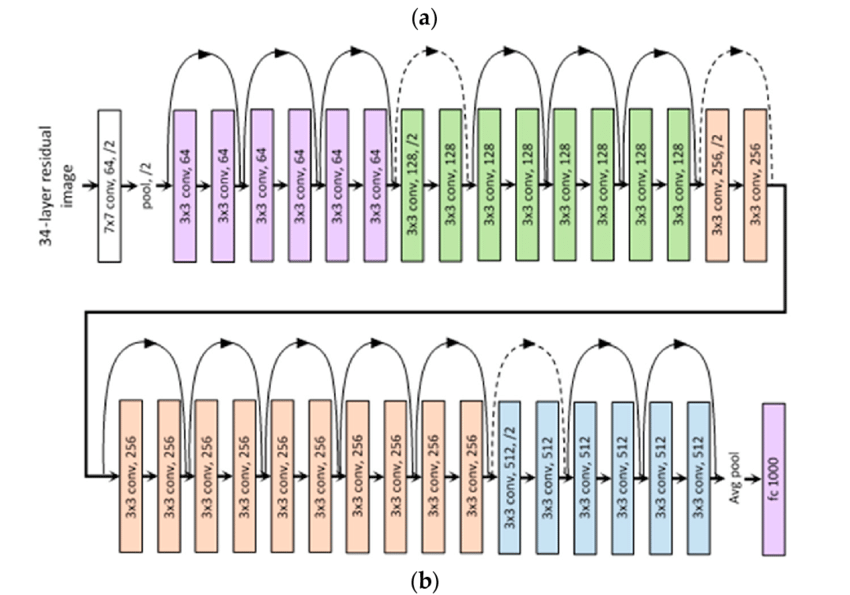
\includegraphics[width=0.45\textwidth]{images/resnet_architecture.png}}\hskip4pt
        \subfloat[Vision Transformer]{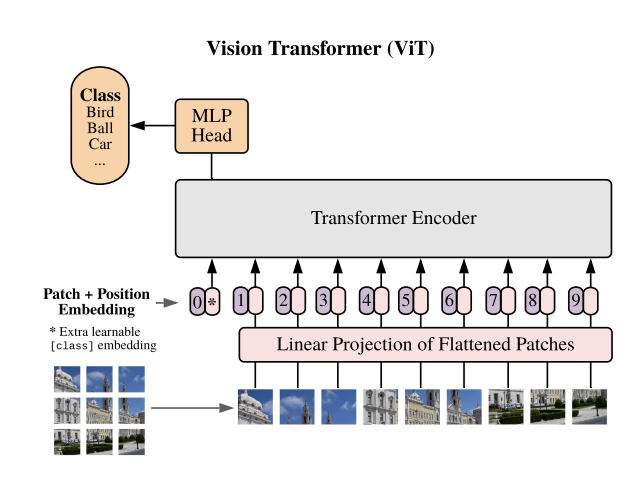
\includegraphics[width=0.45\textwidth]{images/vit_architecture.png}}
    \end{figure}

    \begin{block}{}
        ResNet и Vision Transformer являются самыми показательными моделями из области компьютерного зрения.
    \end{block}
\end{frame}

\section{Методология}

\begin{frame}{Данные}
    Данные сгенерированы с помощью GEANT4. Каждый элемент состоит из:

    \begin{itemize}
        \item Матрица неотрицательных чисел (размерность матрицы  может быть от $10 \times 10$ до $40 \times 40$)
        \item Исходная энергия фотона
        \item Положение входной точки фотона
    \end{itemize}

    \begin{figure}
        \centering
        \subfloat{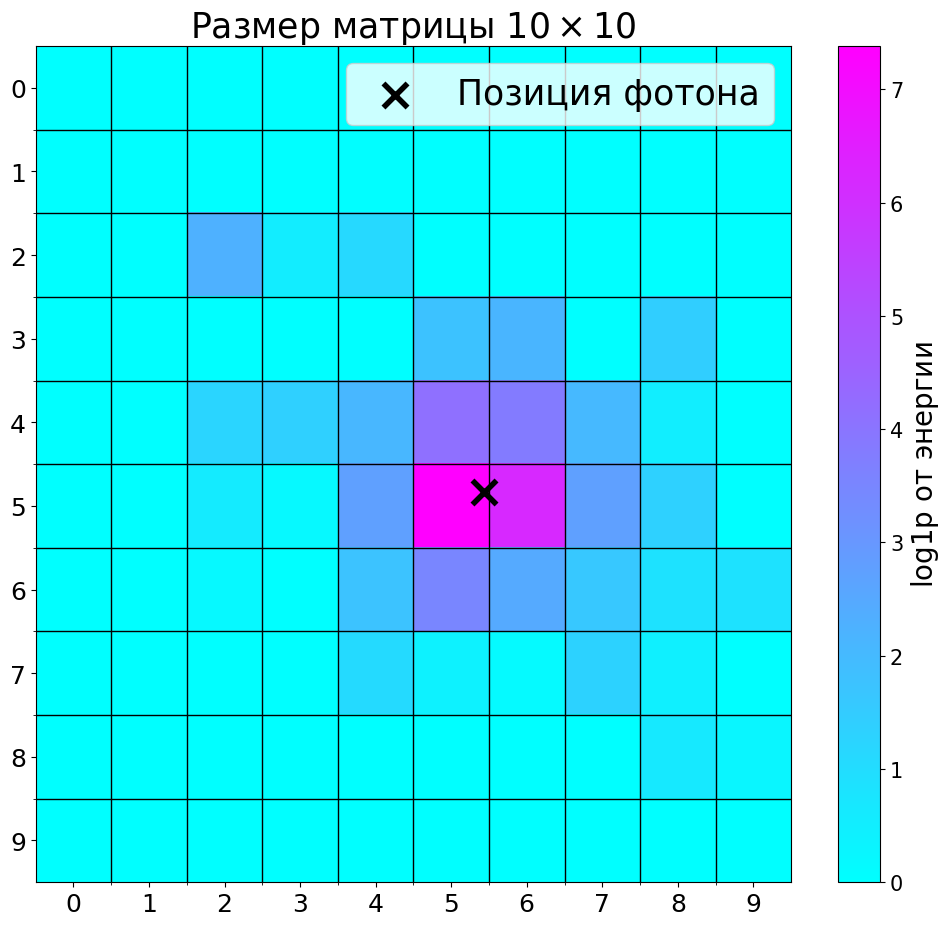
\includegraphics[width=0.4\textwidth]{../report/graphics/data_10x10.png}}\hskip4pt
        \subfloat{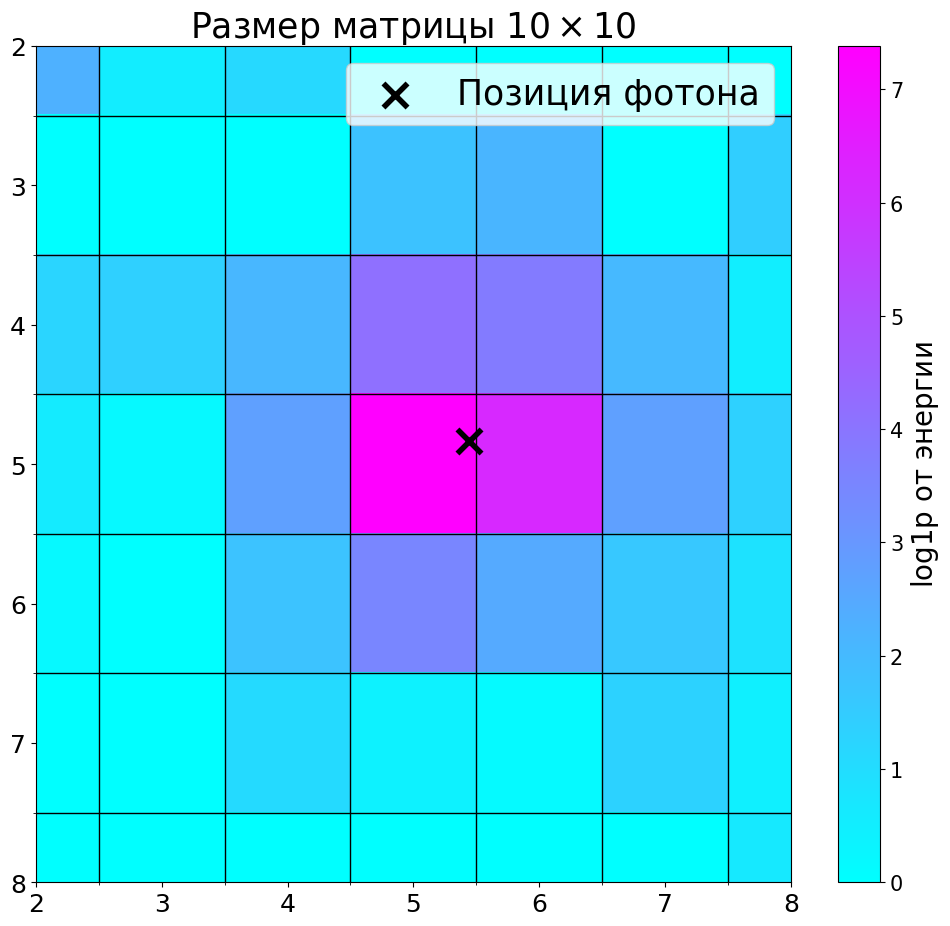
\includegraphics[width=0.4\textwidth]{../report/graphics/data_10x10_zoomed.png}}
    \end{figure}
\end{frame}


\begin{frame}{Аугментации}
    \begin{block}{Применяемые аугментации}
        \begin{itemize}
            \item Случайное горизонтальное или вертикальное отражение
            \item Случайный поворот на угол вида $0^{\circ}$, $90^{\circ}$, $180^{\circ}$ и $270^{\circ}$.
        \end{itemize}
    \end{block}

    \begin{figure}
        \setcounter{subfigure}{0}
        \centering
        \subfloat[Оригинал]{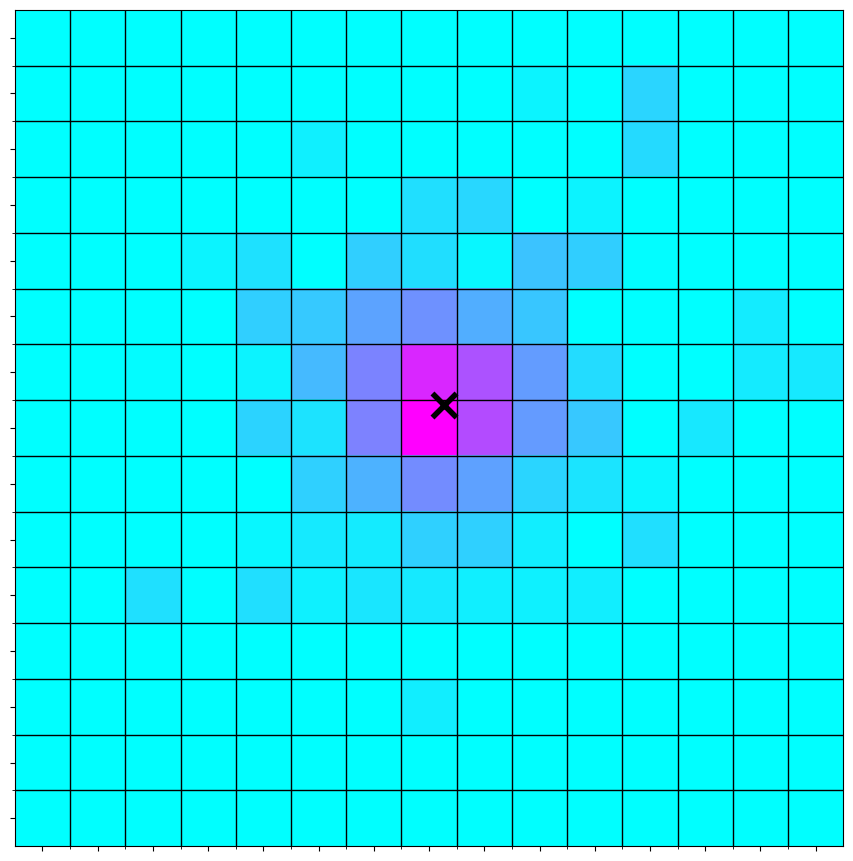
\includegraphics[width=0.32\textwidth]{../report/graphics/data_15x15.png}}\hskip2pt
        \subfloat[Отражение]{\scalebox{-1}[1]{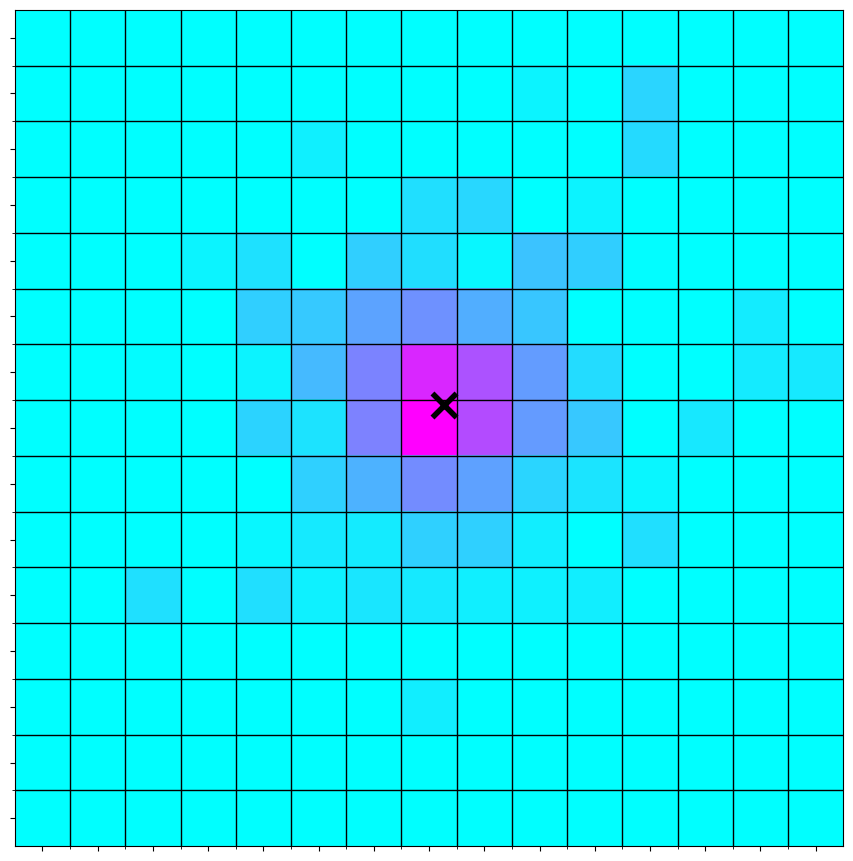
\includegraphics[width=0.32\textwidth]{../report/graphics/data_15x15.png}}}\hskip2pt
        \subfloat[Поворот]{\rotatebox[origin=c]{-90}{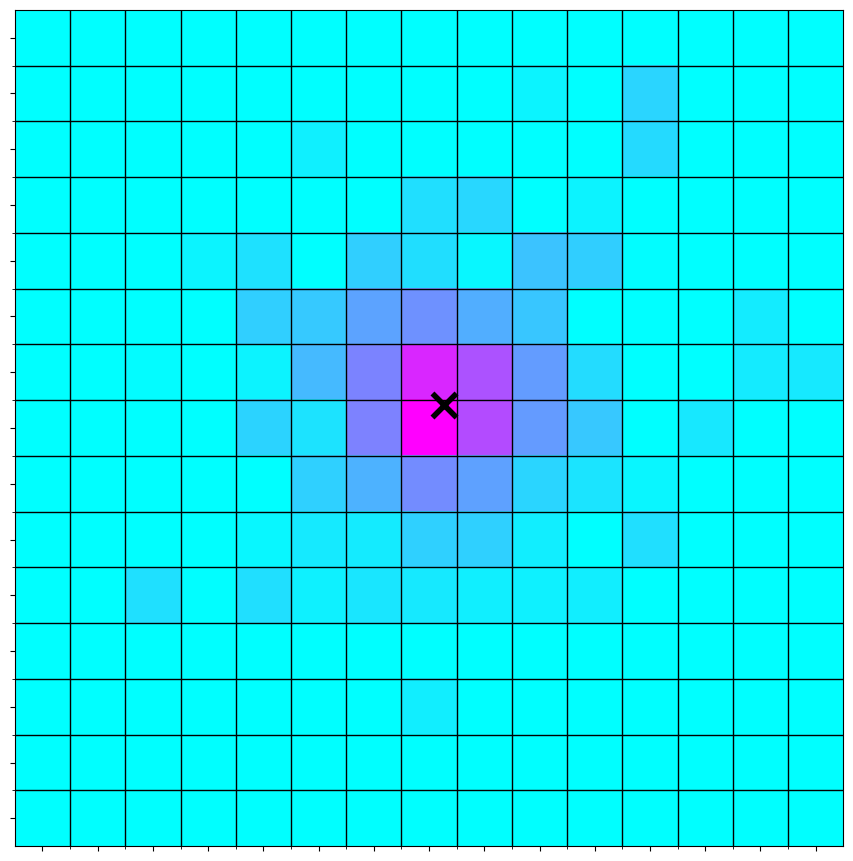
\includegraphics[width=0.32\textwidth]{../report/graphics/data_15x15.png}}}
    \end{figure}
\end{frame}

\begin{frame}{Модели}
    \begin{block}{Использованные модели}
        \begin{itemize}
            \item Аналитическая модель (AnaModel)
            \item Линейная регрессия (LinReg)
            \item ResNet18
            \item Сверточные сети (CNN)
            \item Vision Transformer (ViT)
        \end{itemize}
    \end{block}

    \begin{block}{}
        Модели обучались одновременно на две задачи: реконструкция энергии и восстановление позиции фотона.
        \begin{figure}
            \centering
            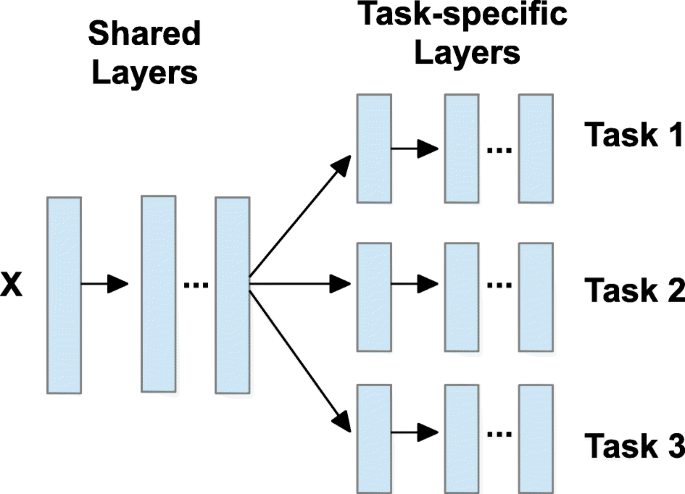
\includegraphics[width=0.35\textwidth]{images/multitask.png}
        \end{figure}
    \end{block}
\end{frame}

\begin{frame}{Метрики}
    \begin{block}{}
        $\{(X_i, E_i, P_i), (\widehat{E}_i, \widehat{P}_i) \}_{i = 1}^{n}$ --- выборка данных, где \begin{itemize}
            \item $X_i$ --- считанные калориметром значения ($\mathbb{R}_{+}^{D \times D}$)
            \item $E_i$ --- исходная энергия фотона ($\mathbb{R}_{+}$)
            \item $P_i = (P_i^x, P_i^y)$ --- позиция входа фотона ($\mathbb{R}^2$)
            \item $\widehat{E}_i$ --- предсказанная энергия ($\mathbb{R}_{+}$)
            \item $\widehat{P}_i = (\widehat{P}_i^x, \widehat{P}_i^y)$ --- предсказанная позиция ($\mathbb{R}^2$)
        \end{itemize}
    \end{block}

    \begin{block}{}
        \begin{align*}
            &\mathcal{L}_{\mathsf{eng}} = \textsf{RMSE/E}(\widehat{E}, E) = \sqrt{\frac{1}{n} \sum_{i = 1}^{n} \left( \frac{\widehat{E}_i - E_i}{E_i} \right)^2} \\
            &\mathcal{L}_{\mathsf{pos}} = \textsf{RMSE}(\widehat{P}, P) = \sqrt{\frac{1}{2 n} \sum_{i = 1}^{n} \left( (\widehat{P}_i^x - P_i^x)^2 + (\widehat{P}_i^y - P_i^y)^2 \right)} \\
            &\mathcal{L}_{\mathsf{total}} = \alpha \cdot \mathcal{L}_{\mathsf{eng}} + (1 - \alpha) \cdot \mathcal{L}_{\mathsf{pos}} , \; \alpha \in [0, 1]
        \end{align*}
    \end{block}
\end{frame}

\section{Результаты}

\begin{frame}{Сравние моделей}
    \begin{figure}
        \centering
        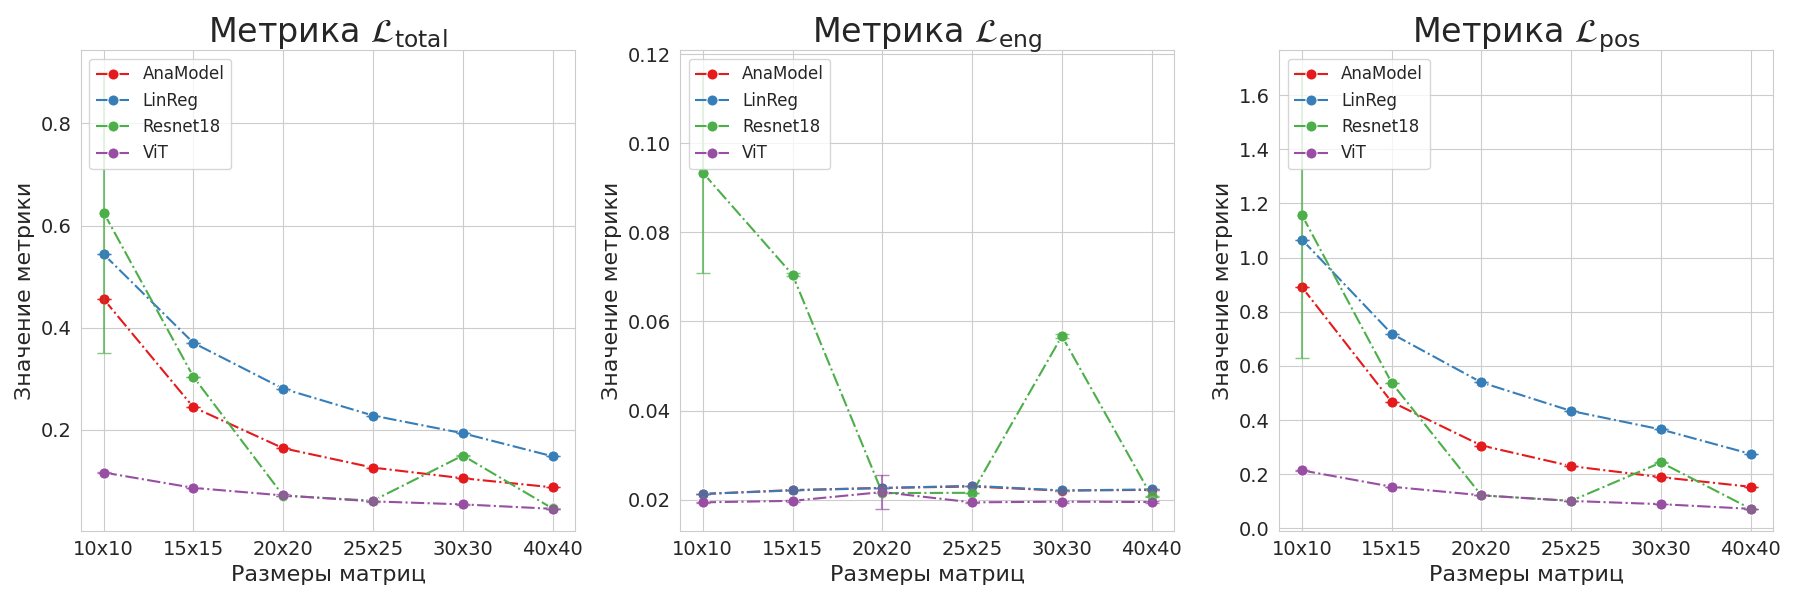
\includegraphics[width=1.0\textwidth]{../report/graphics/models_comp.png}
    \end{figure}

    \begin{block}{}
        Модель ViT показывает лучшие и стабильные результаты.
    \end{block}
\end{frame}

\begin{frame}{Сравние функций потерь}
    \begin{figure}
        \centering
        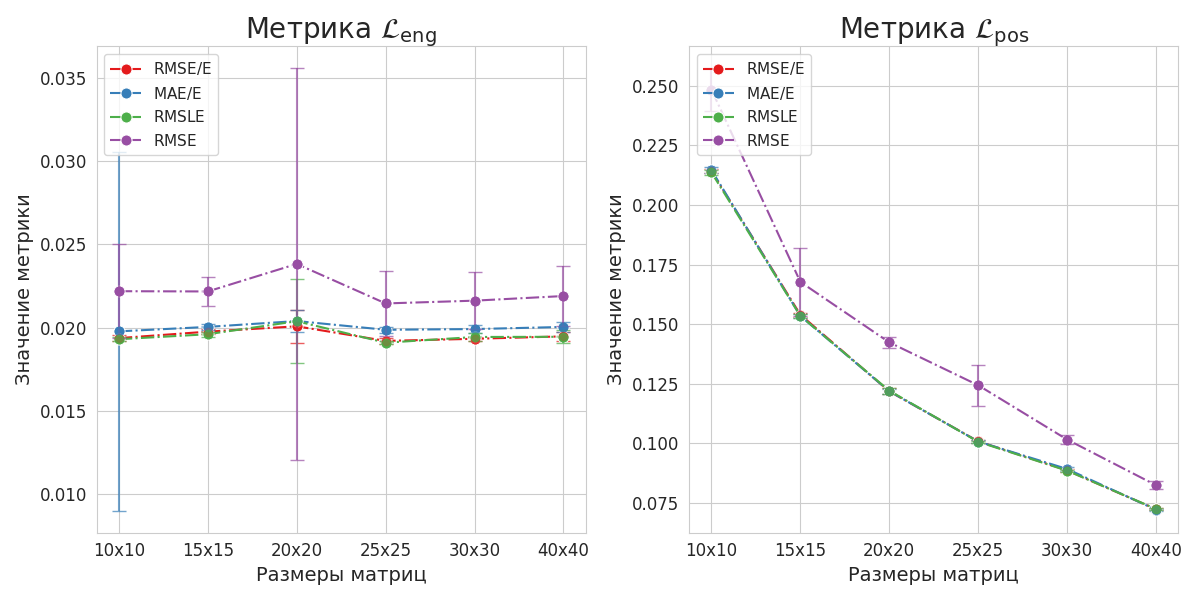
\includegraphics[width=0.9\textwidth]{../report/graphics/loss_comp.png}
    \end{figure}

    \begin{block}{}
        Обучение на нормализованную (относительную) ошибку приводит к лучшему качеству.
    \end{block}
\end{frame}

\begin{frame}{Отношение важности задач}
    \begin{figure}
        \centering
        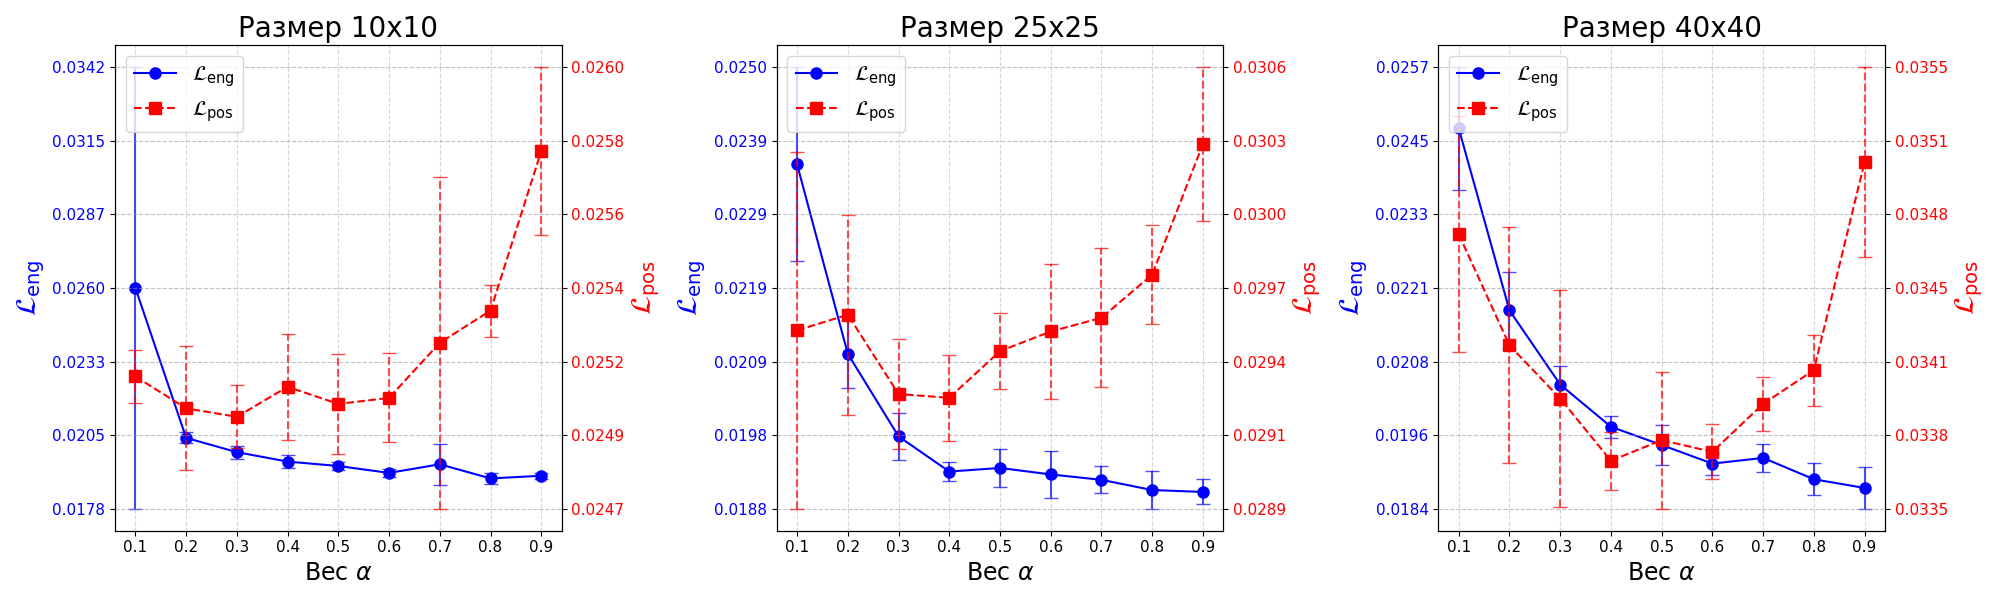
\includegraphics[width=1.0\textwidth]{../report/graphics/exp3_alpha_std.png}
    \end{figure}

    \begin{block}{}
        Влияние гиперпараметра $\alpha$ на качество модели\footnote{$\mathcal{L}_{\mathsf{total}} = \alpha \cdot \mathcal{L}_{\mathsf{eng}} + (1 - \alpha) \cdot \mathcal{L}_{\mathsf{pos}}$.}.
    \end{block}
\end{frame}

\begin{frame}{Размер модели}
    \begin{figure}
        \centering
        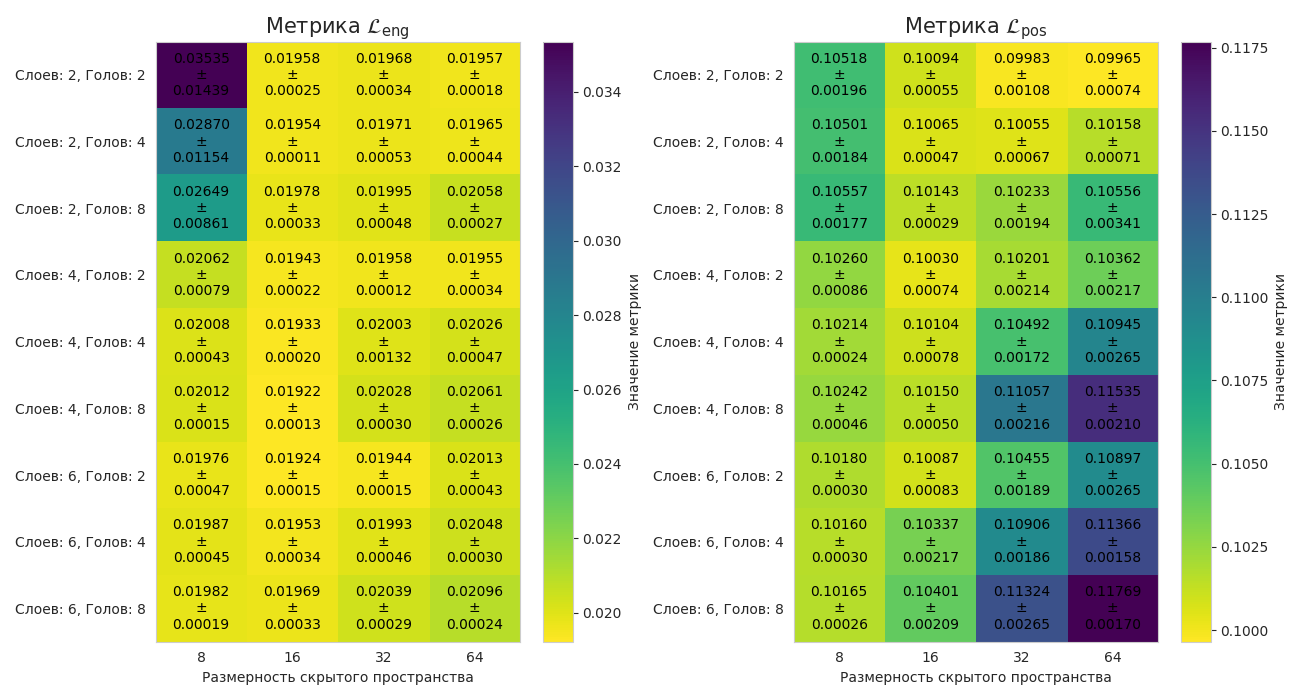
\includegraphics[width=0.9\textwidth]{../report/graphics/exp4_model_params_std.png}
    \end{figure}

    \begin{block}{}
        Оптимальные параметры модели ViT это 4 слоя, 2 головы и размерность скрытого слоя 16.
    \end{block}
\end{frame}

\begin{frame}{Эффективность аугментаций}
    \begin{table}
        \footnotesize
        \centering
        \begin{tabular}{cc|cccc}
            \toprule
            {} & {} & \multicolumn{4}{c}{\textsf{Размер матрицы}} \\
            \cmidrule(lr){3-6}
            {} & {} & \multicolumn{4}{c}{$\mathsf{15 \times 15}$} \\
            \midrule
            \textsf{Отражения} & \textsf{Повороты} & $\mathcal{L}_{\mathsf{eng}}^{\mathsf{train}}$ & $\mathcal{L}_{\mathsf{pos}}^{\mathsf{train}}$ & $\mathcal{L}_{\mathsf{eng}}^{\mathsf{val}}$ & $\mathcal{L}_{\mathsf{pos}}^{\mathsf{val}}$ \\
            \midrule
            \xmark & \xmark & $\mathsf{0.0182}$ & $\mathsf{0.1456}$ & $\mathsf{0.0217}$ & $\mathsf{0.1535}$ \\
            \cmark & \xmark & $\mathsf{0.0186}$ & $\mathsf{0.1481}$ & $\mathsf{0.0194}$ & $\mathsf{0.1537}$ \\
            \xmark & \cmark & $\mathsf{0.0185}$ & $\mathsf{0.1476}$ & $\mathsf{0.0193}$ & $\mathsf{0.1528}$ \\
            \cmark & \cmark & $\mathsf{0.0185}$ & $\mathsf{0.1475}$ & $\mathsf{0.0192}$ & $\mathsf{0.1525}$ \\        
            
            \bottomrule
        \end{tabular}
    \end{table}

    \begin{block}{Применение аугментаций}
        \begin{itemize}
            \item Улучшение качества на валидационной выборке
            \item Сокращение разрыва между обучающей и валидационной выборкой
        \end{itemize}
    \end{block}
\end{frame}

\begin{frame}{Итоговое качество}
    \begin{figure}
        \centering
        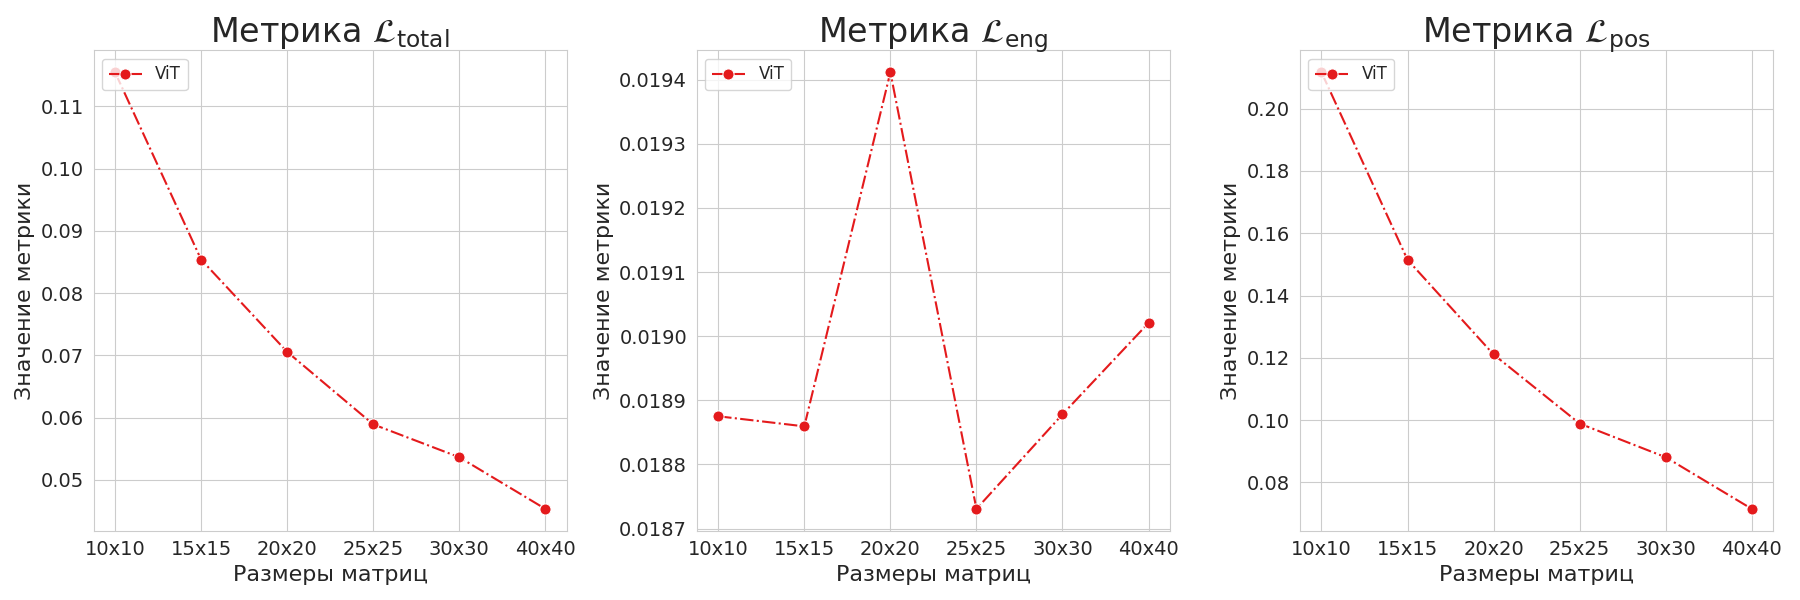
\includegraphics[width=1.0\textwidth]{../report/graphics/best_vit.png}
    \end{figure}

    \begin{block}{Модель ViT одновременно}
        \begin{itemize}
            \item решает задачу восстановления энергии с относительной ошибкой в $1.3\%$
            \item решает задачу реконструкции позиции с точностью, в $20$ раз меньшую размера ячейки калориметра
        \end{itemize}
    \end{block}
\end{frame}

\section{Заключение}

\begin{frame}{Заключение}
    \begin{block}{Пункты на защиту}
        \begin{itemize}
            \item 
        \end{itemize}
    \end{block}
\end{frame}

\begin{frame}[allowframebreaks]
    \frametitle{Список литературы}
    \printbibliography
\end{frame}

\section{Приложения}

\begin{frame}{Метрики}
    \begin{itemize}
        \item Корень из среднеквадратичной ошибки (\textsf{RMSE})
        \item Средняя абсолютная ошибка (\textsf{MAE})
        \item Корень из среднеквадратичной логарифмической ошибки (\textsf{RMSLE}): \[ \textsf{RMSLE}(a, y) = \sqrt{\frac{1}{n} \sum_{i = 1}^{n} (\log(a_i + 1) - \log(y_i + 1))^2} . \]
        \item Взвешенный корень из среднеквадратичной ошибки (\textsf{RMSE/E}): \[ \textsf{RMSE/E}(a, y) = \sqrt{\frac{1}{n} \sum_{i = 1}^{n} \left( \frac{a_i - y_i}{y_i} \right)^2} . \]
        \item Взвешенная средняя абсолютная ошибка (\textsf{MAE/E}): \[ \textsf{MAE/E}(a, y) = \frac{1}{n} \sum_{i = 1}^{n} \frac{|a_i - y_i|}{y_i} . \]
    \end{itemize}
\end{frame}

\begin{frame}{Полное сравнение моделей}
    \begin{figure}
        \centering
        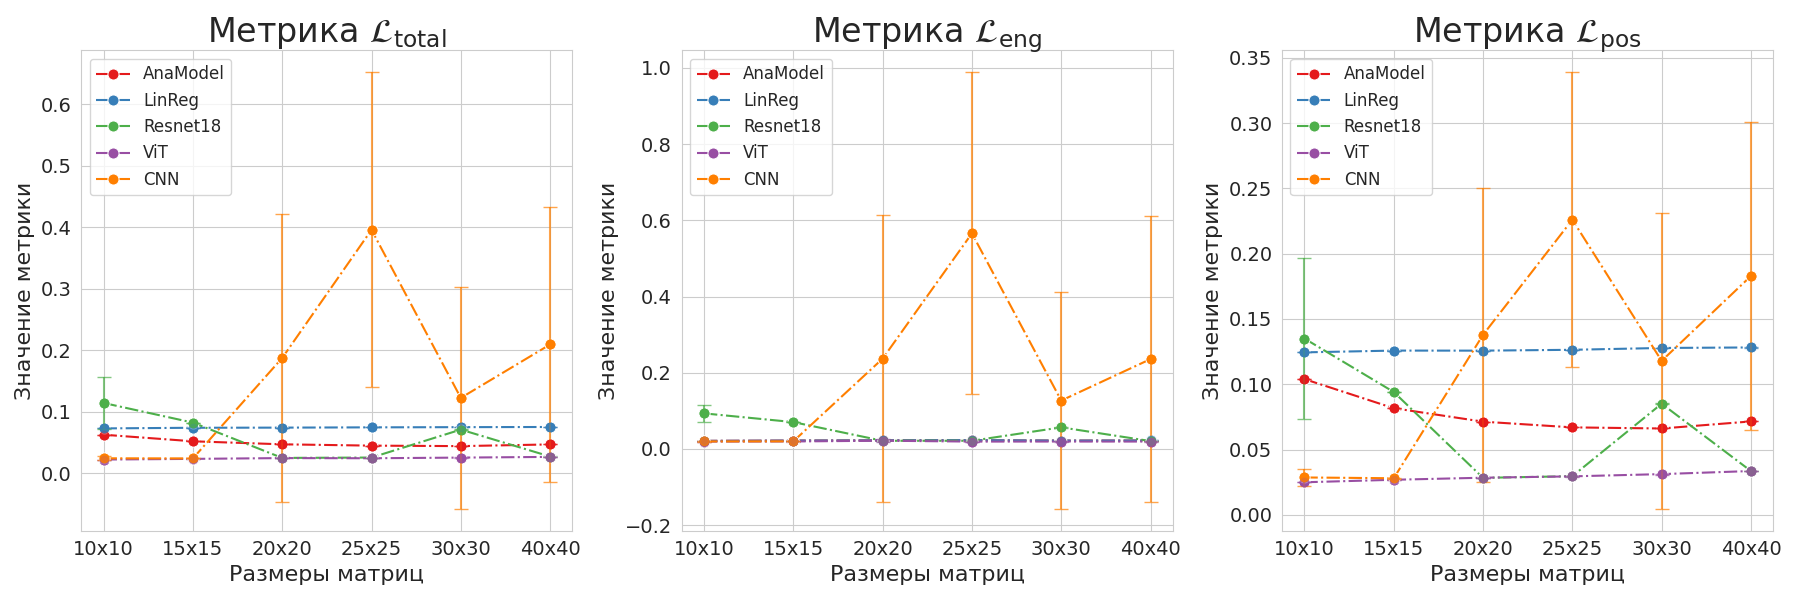
\includegraphics[width=1.0\textwidth]{../report/graphics/models_comp_extra.png}
    \end{figure}

    \begin{block}{}
        Модель CNN показывает слабые результаты, поэтому не была включена в основные слайды.
    \end{block}
\end{frame}

\begin{frame}{Таблица результатов лучшей модели}
    \begin{table}
        \footnotesize
        \centering
        \begin{tabular}{lrrrrrrr}
            \toprule
            {} & \multicolumn{6}{c}{\textsf{Размер матрицы}} \\
            \cmidrule(lr){2-7}
            \textsf{Метрика} & $\mathsf{10 \times 10}$ &  $\mathsf{15 \times 15}$ &  $\mathsf{20 \times 20}$ &  $\mathsf{25 \times 25}$ &  $\mathsf{30 \times 30}$ &  $\mathsf{40 \times 40}$ \\
            \midrule
            $\mathcal{L}_{\mathsf{total}}$ & $\mathsf{0.1153}$ & $\mathsf{0.0852}$ & $\mathsf{0.0702}$ & $\mathsf{0.0588}$ & $\mathsf{0.0535}$ & $\mathsf{0.0453}$ \\
            $\mathcal{L}_{\mathsf{eng}}$ & $\mathsf{0.0189}$ & $\mathsf{0.0189}$ & $\mathsf{0.0194}$ & $\mathsf{0.0187}$ & $\mathsf{0.0189}$ & $\mathsf{0.0190}$ \\
            $\mathcal{L}_{\mathsf{pos}}$ & $\mathsf{0.2117}$ & $\mathsf{0.1515}$ & $\mathsf{0.1211}$ & $\mathsf{0.0989}$ & $\mathsf{0.0881}$ & $\mathsf{0.0715}$ \\
            \textsf{Размер одной ячейки} & $\mathsf{6.0600}$ & $\mathsf{4.0400}$ & $\mathsf{3.0300}$ & $\mathsf{2.4240}$ & $\mathsf{2.0200}$ & $\mathsf{1.5150}$ \\
            $\textsf{MAE/E}_{\textsf{eng}}$ & $\mathsf{0.0131}$ & $\mathsf{0.0127}$ & $\mathsf{0.0132}$ & $\mathsf{0.0124}$ & $\mathsf{0.0130}$ & $\mathsf{0.0129}$ \\        
            \bottomrule
        \end{tabular}
    \end{table}

    \begin{block}{}
        Модель \textsf{ViT} способна решать задачу реконструкции позиции с точностью, в $20$ раз меньшую чем длина стороны центральной ячейки. Более того, данная модель решает задачу восстановления энергии с относительной ошибкой в $1.3\%$.
    \end{block}
\end{frame}

\end{document}